% Issue 12 draft, 24 November 2026. Review/source map: Issue 12.
% Issue 9.1: corpus-description addition approved; existing Results preserved.
% Transfer-network structure: approved by the user, including tone/explanation.
% Premier League entry by age: approved by the user.
% Guardian coverage volume: approved, with the short zero-coverage clarification.
% Measuring tone in football writing: approved, including revised averaging text.
% Changes in Guardian tone by age: approved by the user.
% All five Results subsections are approved; compiled fit remains for Issues 13--14.
% Template assembly, bibliography integration and compilation: Issues 13--14.
\section*{Results}

\subsection*{Transfer-network structure}

We first represented eligible transfers as a directed network, with clubs as nodes and origin--destination routes weighted by the number of transfers. The 16,636 transfers involving 4,602 players in recorded seasons 2012/13--2024/25 connected 1,157 clubs through 11,016 routes.

Figure~\ref{fig:entry-age}(a) shows a filtered view of this network using a disparity cutoff of $\alpha = 0.20$ \cite{serrano2009multiscale}. The backbone retained 383 clubs and 1,396 routes carrying 5,271 transfers (31.7\% of the sample). Colours and shapes identify five communities found by directed Louvain on the full network \cite{blondel2008louvain,dugue2015directed}. This view pools both age groups and includes Premier League and other destinations. The entry-by-age comparison below uses the full transfer sample.

We also explored Leiden, a refinement of the widely used Louvain method that addresses problems with community connectivity \cite{traag2019leiden}. Its original evaluation reported faster runtime than Louvain. Both methods identified five communities in the observed network, with broadly similar club memberships. Modularity was higher in the observed network than in the same randomized network for both Leiden (0.448 versus 0.215) and Louvain (0.446 versus 0.213). By this measure, transfer activity was more strongly concentrated within communities in the observed network.

\subsection*{Premier League entry by age}

We compared the share of eligible transfers entering the Premier League for the two age groups (Figure~\ref{fig:entry-age}(b)). To assess the gap, we shuffled age labels among transfers from the same origin club and recorded season, keeping destinations fixed.

Among eligible recorded transfers in source seasons 2012/13--2024/25, 12.14\% of transfers involving players aged 30+ entered the Premier League, compared with 14.56\% for players under 30 (gap $-2.42$ percentage points). The observed gap was more negative than the mean within-origin-club/season permutation gap ($-1.31$ points), but evidence against this null was limited (one-sided p = 0.098).

Players can make several transfers over their careers, so frequent movers contribute more observations to the main analysis and may disproportionately influence the comparison between age groups. As a sensitivity check, we selected one eligible transfer uniformly at random for each player and repeated the permutation analysis on this fixed sample. This gave every eligible player equal representation, allowing us to examine whether the observed age difference also appeared after removing repeated contributions. In this sample of 4,602 players, joining rates remained lower for transfers involving players aged 30+ (19.52\% versus 21.46\%; gap $-1.94$ percentage points; one-sided p = 0.074). The result is conditional on this one selection and does not assess variation across alternative selections.

\subsection*{Guardian coverage volume}

We examined Guardian coverage in a separate sample of 1,332 selected Premier League signings. The collected coverage included 43,924 distinct articles before sentiment filters were applied. To describe attention around each signing, we counted distinct articles naming the player before and after the move, including all article types.

Older signings received more Guardian coverage in both periods. The median number of distinct articles per signing was 27.5 for players aged 30+ versus 12 for those under 30 before signing, and 47.5 versus 35 after signing. Counts include signings with no recorded coverage.

\subsection*{Measuring tone in football writing}

For the tone comparison, a signing needed at least five scored sentences both before and after the move, after excluding liveblogs and match reports. This left 820 signings: 67 involving players aged 30+ and 753 involving younger players.

The selected corpus comprised 99,976 linked sentence records, containing 3.87 million tokens and 42,779 token types, of which 13,022 were hapax tokens. Table~\ref{tab:guardian-tokens} lists the ten most frequent tokens in each ranking, with and without stopwords. After removing stopwords, frequent tokens included ``season'', club-name components such as ``city'' and ``united'', and ``form'', ``injured'' and ``unknown''. Figure~\ref{fig:guardian-rank-frequency} shows frequency rank and raw counts with stopwords on logarithmic axes, with an ideal Zipf reference ($s = 1$) anchored to the most frequent token. Counts lay above this reference for many common tokens and below it for the rarest tokens. These counts partly describe the vocabulary of the selected corpus. The following analysis examines the tone of the sentences.

We applied four scoring methods to player-linked sentences, including quotations: RoBERTa \cite{liu2019roberta,loureiro2022timelms,camachocollados2022tweetnlp,cardiffnlp2022checkpoint}, VADER \cite{hutto2014vader}, the Bing opinion lexicon \cite{hu2004mining}, and Bing excluding 21 football-related words. Higher scores indicate more positive language. For the overall before--after comparison, we averaged all available sentence scores for each signing separately before and after the move. The monthly curves in Figure~\ref{fig:h2-monthly-tone} were calculated separately, using sentence scores from each month. These scores describe how the selected published sentences read; they do not directly identify the journalist's attitude toward the player.

To check the scores against human judgments, one author labelled 200 sentences. Four wrong-person matches were excluded, leaving 196 evaluable sentences.

Table~\ref{tab:validation} checks three aspects of the sentence scores. The human labels were ordered from negative to neutral to positive, with all sentences in each category sharing a rank. Spearman's $\rho$ compares those category ranks with the ranks of each model's numerical scores. A positive $\rho$ indicates that the model's ranking tended to agree with the order of the three categories. Correct sign measures whether scores are above zero for human-positive sentences and below zero for human-negative sentences, excluding human-neutral cases. Three-class accuracy measures exact agreement with positive, neutral or negative labels across all sentences. RoBERTa had the strongest observed rank agreement ($\rho = 0.52$, 95\% bootstrap interval 0.38--0.63) and the correct sign for 70 of 85 positive or negative sentences (82\%). Its three-class predictions matched 98 of 196 labels (50\%), showing the difficulty of distinguishing neutral language. These checks support using RoBERTa as a useful but imperfect measure; the 14 older-player sentences leave age-specific comparability uncertain.

% Approved Table 1 values, caption and note, 24 November 2026.
% Native LaTeX transcription for Issue 12; compiled layout checked in Issues 13--14.
\begin{table}[tbhp]
\centering
\small
\setlength{\tabcolsep}{4.5pt}
\caption{Agreement of four sentiment instruments with human judgments of Guardian sentences.}
\label{tab:validation}
\begin{tabular}{lccc}
\toprule
Instrument & $\rho$ (95\% CI) & Sign right & 3-class accuracy \\
\midrule
RoBERTa & 0.52 (0.38, 0.63) & 82\% & 50\% \\
VADER & 0.33 (0.21, 0.45) & 68\% & 42\% \\
Bing & 0.36 (0.22, 0.47) & 59\% & 51\% \\
Bing, no football words & 0.36 (0.23, 0.49) & 58\% & 53\% \\
\bottomrule
\end{tabular}
\addtabletext{Results use 196 hand-labelled sentences after excluding four wrong-person matches. Spearman's $\rho$ measures whether sentences judged more positive receive higher scores; 95\% confidence intervals use 2,000 sentence bootstrap resamples. Correct sign is the percentage of the 85 human-positive or human-negative sentences whose score has the corresponding sign. Three-class accuracy is the percentage of all 196 sentences classified correctly as positive, neutral or negative. Neutral scores fall within $\pm0.05$ for RoBERTa and VADER and equal zero for both Bing variants. Only 14 sentences concern players aged 30+, leaving age-specific validity uncertain.}
\end{table}


\guardianSentimentFigure
\subsection*{Changes in Guardian tone by age}

Figure~\ref{fig:h2-monthly-tone} shows monthly mean sentence sentiment for older and younger signings, separately for RoBERTa, VADER and the two Bing variants. For each signing, we first averaged the sentiment scores of the sentences published in a given month. We then averaged these monthly values separately for older and younger signings. Only signings with sentences in a month contributed to that month's average. The curves show these monthly group means smoothed with a centred three-month moving average, separately before and after signing.

First, we calculated one tone change per signing by subtracting its mean sentiment score before the move from its mean score after the move. We averaged these changes within each age group, giving every signing equal weight. With RoBERTa, the mean change was $-0.0076$ for the 30+ group and $-0.0137$ for the under-30 group. Subtracting the younger group's mean change from the older group's, using unrounded values, gave a gap of +0.0060 score units.

We kept each signing's tone change fixed and shuffled the age-group labels within each season 5,000 times, recalculating the gap after each shuffle. We found no clear evidence that sentiment changed differently for older and younger signings. VADER and both Bing variants also provided no clear evidence of different changes.

\subsection*{Sub-analysis of the transfer network}

During the network analysis, we also examined which club pairs accounted for unusually many transfers among the 2,396 Premier League arrivals. The exploratory screen selected 217 recurring routes, each with at least two recorded transfers, accounting for 626 transfers (Figure~\ref{fig:feeder-routes}). Girona to Manchester City was the busiest transfer pair, with 15 recorded transfers over the study period. We calculated an expected count for that route in each season, keeping fixed how many transfers each origin club sent to the Premier League and how many each destination club received. Adding those seasonal expectations gave an expected total of 1.8 transfers across the full 2012/13--2024/25 period.

We found that some high-volume transfer pairs shared a common equity investor. The 17 transfer pairs in the joint-ownership group had a median of four transfers. In comparison, the remaining 200 transfer pairs had a median of two (Figure~\ref{fig:feeder-routes}b).

\begin{figure*}[!t]
  \centering
  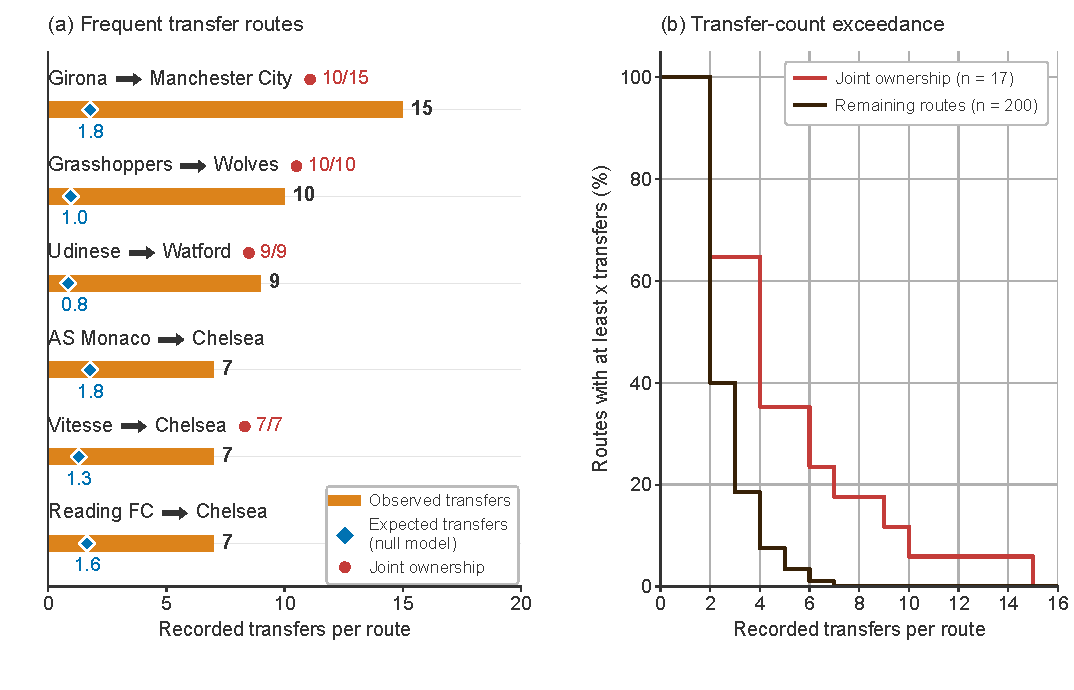
\includegraphics[trim=16bp 20bp 0bp 3bp,clip,width=0.80\textwidth]{../reruns/h1_2012_13-2024_25/output/premier_league_feeder_findings_three_panel.pdf}
  \caption{\textbf{Recurring transfer routes into the Premier League.} \textbf{(a)} The six screened transfer pairs with at least seven recorded transfers among 2,396 arrivals in recorded seasons 2012/13--2024/25. Bars show observed counts and diamonds show expectations under the seasonal destination shuffle. For Girona and Udinese, the red fractions show how many of each route's transfers occurred during documented joint ownership. \textbf{(b)} The exceedance curves show the percentage of routes in each group with at least a given number of recorded transfers.}
  \label{fig:feeder-routes}
\end{figure*}
